%!TEX program = xelatex
\documentclass{beamer}
\usepackage{pc_slides}
\usepackage[backend=bibtex, url=false, doi=false, isbn=false, eprint=false]{biblatex}
\bibliography{/Users/phil/bibs/library.bib}{}
\renewcommand{\footnotesize}{\tiny}
\usepackage{bbm}


\title{What's Going on with Scale-Free Networks?}
% \subtitle{6.268, Lecture 8}
\date{\today}
\author{Phil Chodrow}
\institute{MIT  Operations Research Center \\ Human Mobility and Networks Laboratory  \\ Laboratory for Information and Decision Systems}
\graphicspath{{../figs/}}
% -------------------------------------------------------------------------------------------------
% -------------------------------------------------------------------------------------------------
% -------------------------------------------------------------------------------------------------

\newcommand\abs[1]{\left|#1\right|}
\newcommand\E[0]{\mathbb{E}}
\newcommand\prob[0]{\mathbb{P}}
\newcommand\R[0]{\mathbb{R}}


\begin{document}

% \def\short{1}

\newif\iflong
\ifdefined\short
	\longfalse
\else
	\longtrue
\fi

\maketitle

\section{What's Going On?}
	%%%%%%%%%%%%%%%%%%%%%%%%%%%%%%%%%%%%%%%%%%%%%%%%%%%%%%%%%%%%%%%%%%%%%%%%%%%%%%%%%%%%%%%%%%%
		
		\begin{frame}\frametitle{Media Coverage}
			\centering
		  	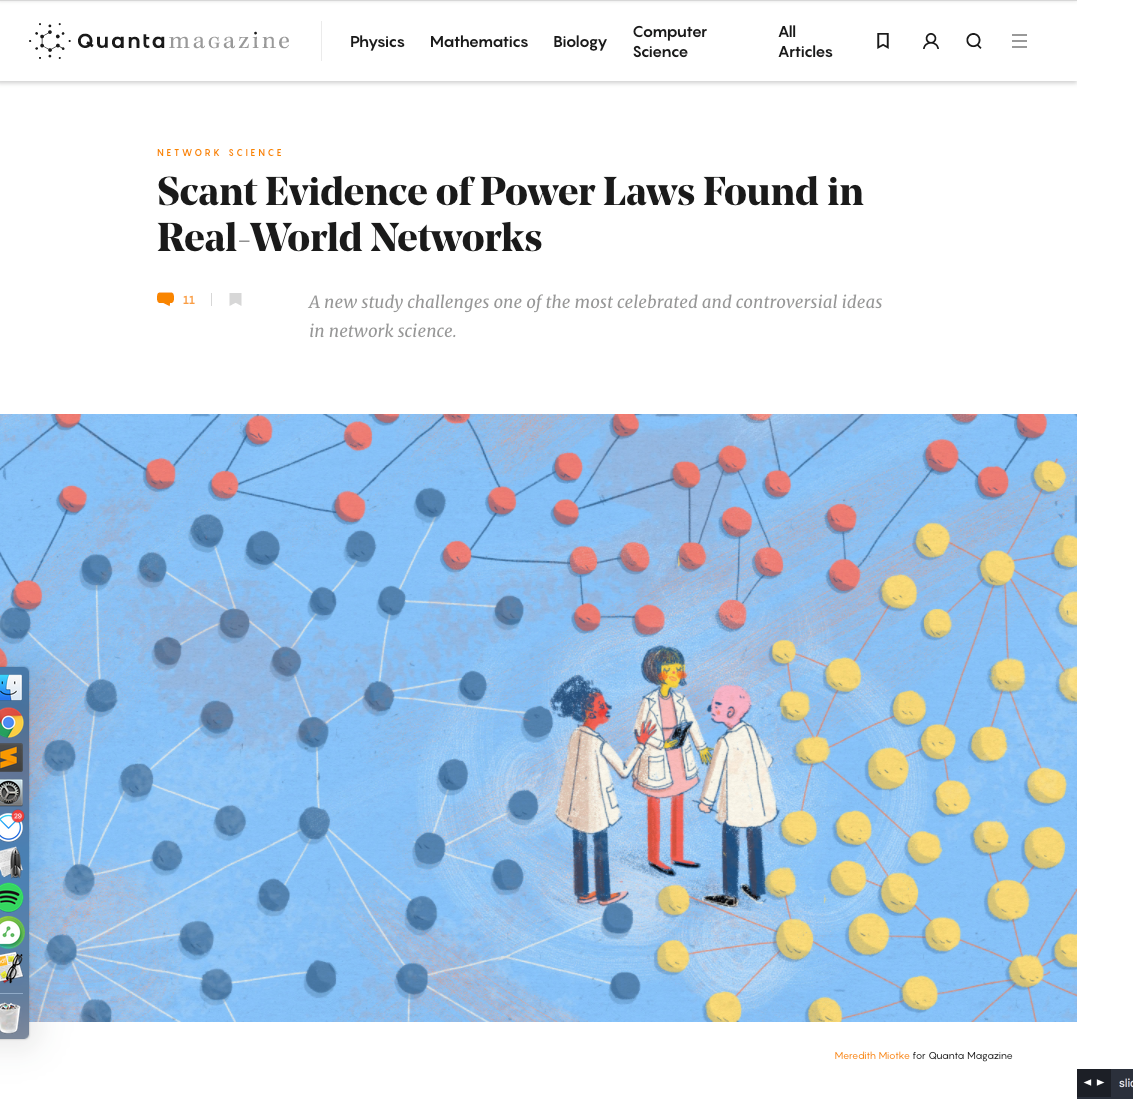
\includegraphics[width=.7\textwidth]{quanta}
		\end{frame}

	%%%%%%%%%%%%%%%%%%%%%%%%%%%%%%%%%%%%%%%%%%%%%%%%%%%%%%%%%%%%%%%%%%%%%%%%%%%%%%%%%%%%%%%%%%%
	%%%%%%%%%%%%%%%%%%%%%%%%%%%%%%%%%%%%%%%%%%%%%%%%%%%%%%%%%%%%%%%%%%%%%%%%%%%%%%%%%%%%%%%%%%%
		
		\begin{frame}\frametitle{Weird Blog Posts}
		  	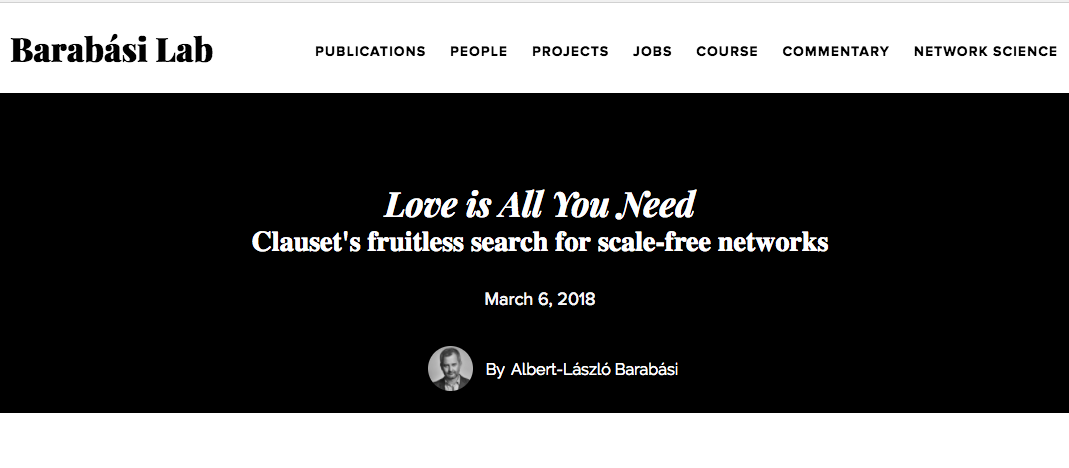
\includegraphics[width=\textwidth]{love}
		\end{frame}

	%%%%%%%%%%%%%%%%%%%%%%%%%%%%%%%%%%%%%%%%%%%%%%%%%%%%%%%%%%%%%%%%%%%%%%%%%%%%%%%%%%%%%%%%%%%
	%%%%%%%%%%%%%%%%%%%%%%%%%%%%%%%%%%%%%%%%%%%%%%%%%%%%%%%%%%%%%%%%%%%%%%%%%%%%%%%%%%%%%%%%%%%
		
		\begin{frame}\frametitle{Twitter Fights}
		  	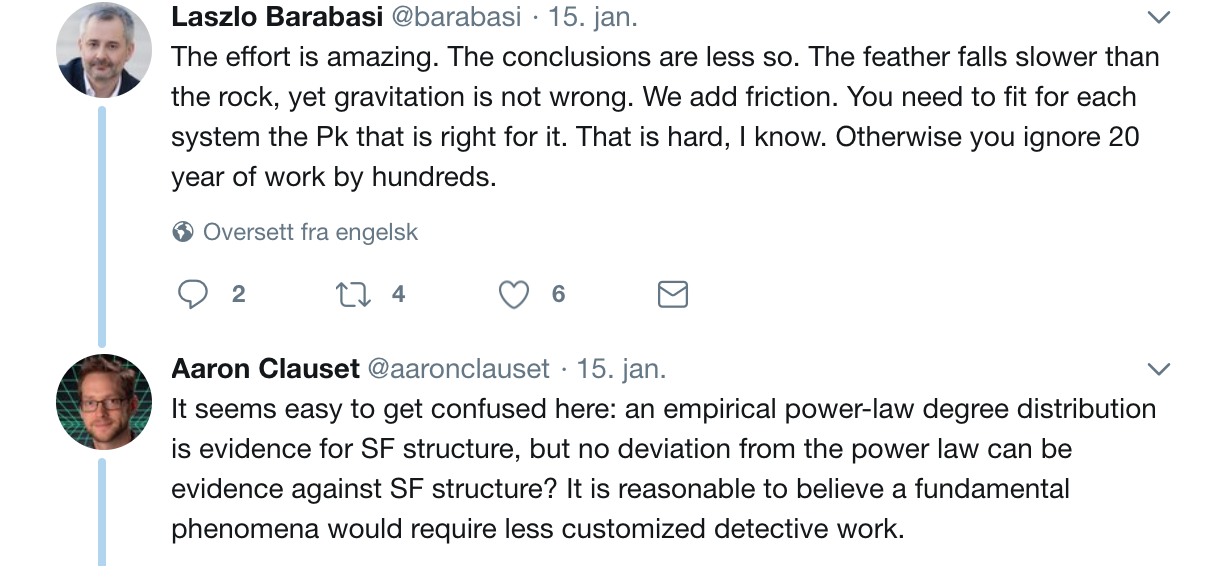
\includegraphics[width=\textwidth]{twitter}
		\end{frame}

	%%%%%%%%%%%%%%%%%%%%%%%%%%%%%%%%%%%%%%%%%%%%%%%%%%%%%%%%%%%%%%%%%%%%%%%%%%%%%%%%%%%%%%%%%%%
	%%%%%%%%%%%%%%%%%%%%%%%%%%%%%%%%%%%%%%%%%%%%%%%%%%%%%%%%%%%%%%%%%%%%%%%%%%%%%%%%%%%%%%%%%%%
		
		\begin{frame}[standout]
		  	Ummmm....What are we talking about?
		\end{frame}

	%%%%%%%%%%%%%%%%%%%%%%%%%%%%%%%%%%%%%%%%%%%%%%%%%%%%%%%%%%%%%%%%%%%%%%%%%%%%%%%%%%%%%%%%%%%
\section{A Brief History....}
	%%%%%%%%%%%%%%%%%%%%%%%%%%%%%%%%%%%%%%%%%%%%%%%%%%%%%%%%%%%%%%%%%%%%%%%%%%%%%%%%%%%%%%%%%%%
	%%%%%%%%%%%%%%%%%%%%%%%%%%%%%%%%%%%%%%%%%%%%%%%%%%%%%%%%%%%%%%%%%%%%%%%%%%%%%%%%%%%%%%%%%%%
		
		\begin{frame}\frametitle{The Setting}
		  	\begin{itemize}
		  		\pause \item It's the late 1990s. 
		  		\pause \item The work of Erd\"{o}s and Renyi is still the \textbf{dominant paradigm} for thinking about and modeling networks. 
		  		\pause \item But \textbf{digital infrastructure} and \textbf{computing power} are growing...
		  		\pause \item For the first time, we can \textbf{observe} and \textbf{analyze} large networks in the real world. 
		  	\end{itemize}
		\end{frame}
	%%%%%%%%%%%%%%%%%%%%%%%%%%%%%%%%%%%%%%%%%%%%%%%%%%%%%%%%%%%%%%%%%%%%%%%%%%%%%%%%%%%%%%%%%%%
	%%%%%%%%%%%%%%%%%%%%%%%%%%%%%%%%%%%%%%%%%%%%%%%%%%%%%%%%%%%%%%%%%%%%%%%%%%%%%%%%%%%%%%%%%%%
		
		\begin{frame}\frametitle{Network Analysis}
		\centering
			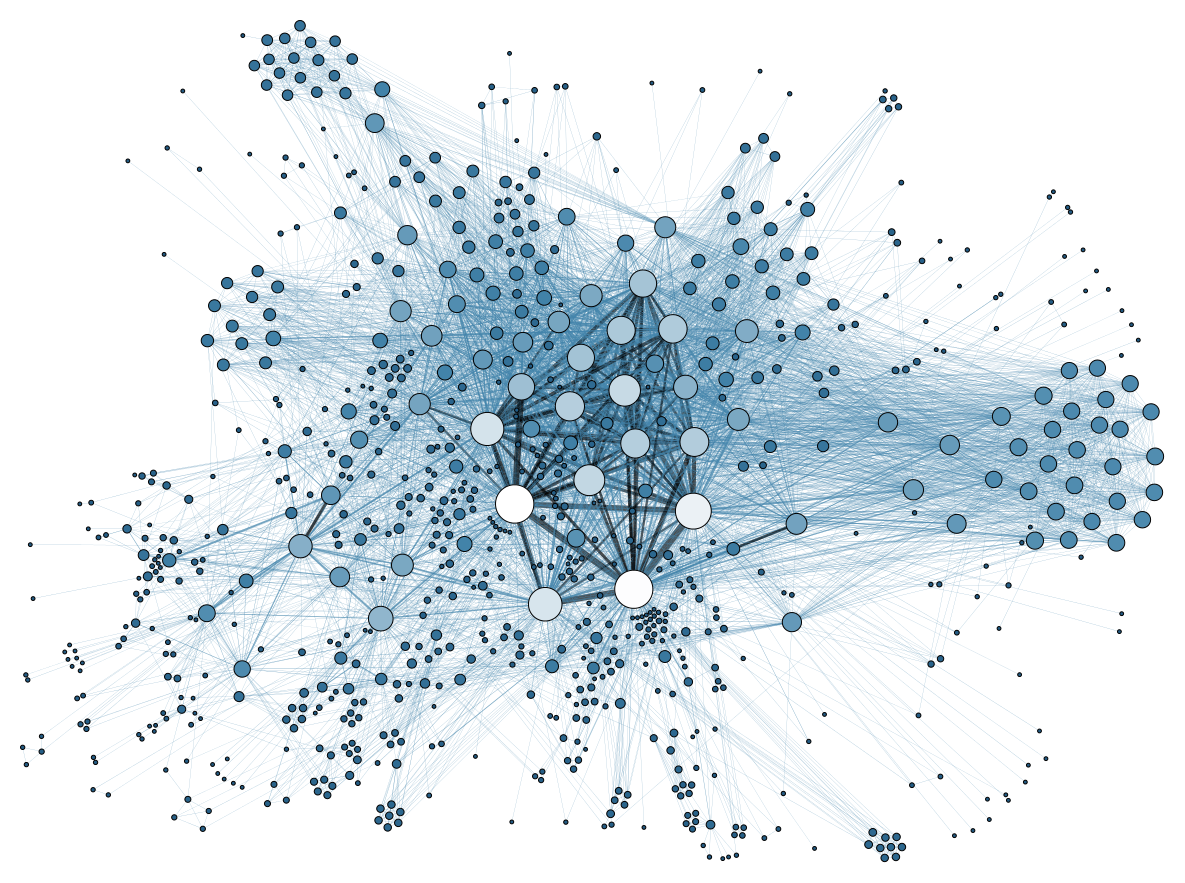
\includegraphics[width=.8\textwidth]{Social_Network_Analysis_Visualization}

		  	Grandjean, Martin (2014). "La connaissance est un réseau". Les Cahiers du Numérique 10 (3): 37-54. DOI:10.3166/LCN.10.3.37-54.
		\end{frame}
	
	%%%%%%%%%%%%%%%%%%%%%%%%%%%%%%%%%%%%%%%%%%%%%%%%%%%%%%%%%%%%%%%%%%%%%%%%%%%%%%%%%%%%%%%%%%%
	%%%%%%%%%%%%%%%%%%%%%%%%%%%%%%%%%%%%%%%%%%%%%%%%%%%%%%%%%%%%%%%%%%%%%%%%%%%%%%%%%%%%%%%%%%%
		\begin{frame}\frametitle{Erd\"{o}s-Renyi Graphs Don't Fit!}
		  	\begin{enumerate}
		  		\pause \item Real networks have high clustering coefficients $\implies$ Watts + Strogatz small world model.\footfullcite{Strogatz1998b}
		  		\pause \item Real networks have highly heterogeneous \emph{degree distributions} -- heavier tails than Poisson. 
		  	\end{enumerate}
		\end{frame}
	
	%%%%%%%%%%%%%%%%%%%%%%%%%%%%%%%%%%%%%%%%%%%%%%%%%%%%%%%%%%%%%%%%%%%%%%%%%%%%%%%%%%%%%%%%%%%
	%%%%%%%%%%%%%%%%%%%%%%%%%%%%%%%%%%%%%%%%%%%%%%%%%%%%%%%%%%%%%%%%%%%%%%%%%%%%%%%%%%%%%%%%%%%
		
		\begin{frame}\frametitle{Emergence of Scaling in Random Networks}
			\begin{figure}
				\centering
				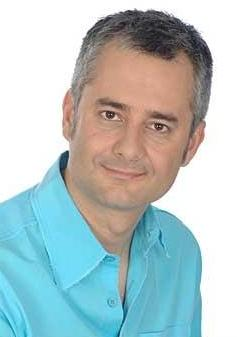
\includegraphics[width=.3\textwidth]{barabasicropped}
				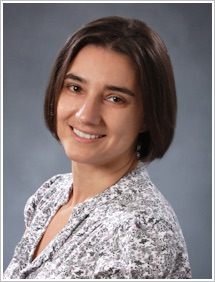
\includegraphics[width=.3\textwidth]{ralbert-photo}
			\end{figure}

			Albert-Laszlo Barabasi + Reka Albert (1999-2002); R.A.'s PhD thesis work.
			
			\pause Central claim: \textbf{many real-world networks are scale-free.}
		
		
		\end{frame}

	%%%%%%%%%%%%%%%%%%%%%%%%%%%%%%%%%%%%%%%%%%%%%%%%%%%%%%%%%%%%%%%%%%%%%%%%%%%%%%%%%%%%%%%%%%%
	%%%%%%%%%%%%%%%%%%%%%%%%%%%%%%%%%%%%%%%%%%%%%%%%%%%%%%%%%%%%%%%%%%%%%%%%%%%%%%%%%%%%%%%%%%%
		
		\begin{frame}\frametitle{Mathematical Definition}
			Discrete random variable $K$ has a \textbf{power law tail} if  
			\begin{align*}
				\prob(K = k) \approx c k^{-\gamma}
			\end{align*}
			for some $\gamma > 1$ and ``sufficiently large'' $k$.
			Formally, 
			\begin{align*}
				\lim_{k \rightarrow \infty} k^\gamma \prob(K = k) = c\;.
			\end{align*}
			Note that $\Theta(k^{-\gamma}) \gg \Theta(e^{-k}) \gg \Theta(e^{-k^2})$. 
		\end{frame}

	%%%%%%%%%%%%%%%%%%%%%%%%%%%%%%%%%%%%%%%%%%%%%%%%%%%%%%%%%%%%%%%%%%%%%%%%%%%%%%%%%%%%%%%%%%%
	%%%%%%%%%%%%%%%%%%%%%%%%%%%%%%%%%%%%%%%%%%%%%%%%%%%%%%%%%%%%%%%%%%%%%%%%%%%%%%%%%%%%%%%%%%%
		
		\begin{frame}\frametitle{The Log-Log Plot}
		  	Power law tails look \textbf{linear} on \textbf{log-log} axes. 
		  	\begin{columns}
		  		\begin{column}{.45\textwidth}
		  			\begin{align*}
		  				\prob(K = k) &\approx c k^{-\gamma} \\ 
		  				\log \prob(K = k) &\approx -\gamma \log k + \log c\;.
		  			\end{align*}
		  		\end{column}
			  	\begin{column}{.55\textwidth}
			  	\begin{figure}
			  		\centering
			  		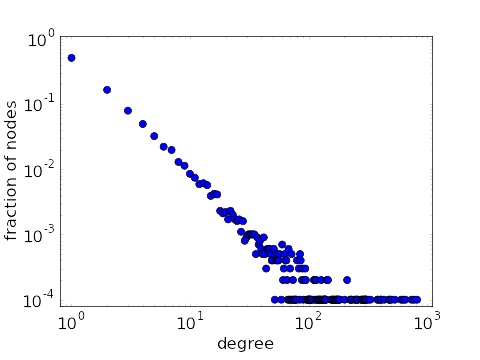
\includegraphics[width=\textwidth]{pl_scatter}
			  		\caption{} \label{fig:}
			  	\end{figure}
			  	\end{column}
		  	\end{columns}
		  	Is everything that looks linear on log-log axes a power law?...
		\end{frame}
	
	%%%%%%%%%%%%%%%%%%%%%%%%%%%%%%%%%%%%%%%%%%%%%%%%%%%%%%%%%%%%%%%%%%%%%%%%%%%%%%%%%%%%%%%%%%%
	%%%%%%%%%%%%%%%%%%%%%%%%%%%%%%%%%%%%%%%%%%%%%%%%%%%%%%%%%%%%%%%%%%%%%%%%%%%%%%%%%%%%%%%%%%%
		
		\begin{frame}\frametitle{\alert{Scale Free} Networks Have \alert{Power Law} Degree Distributions}
		  \begin{figure}
		  	\centering
		  	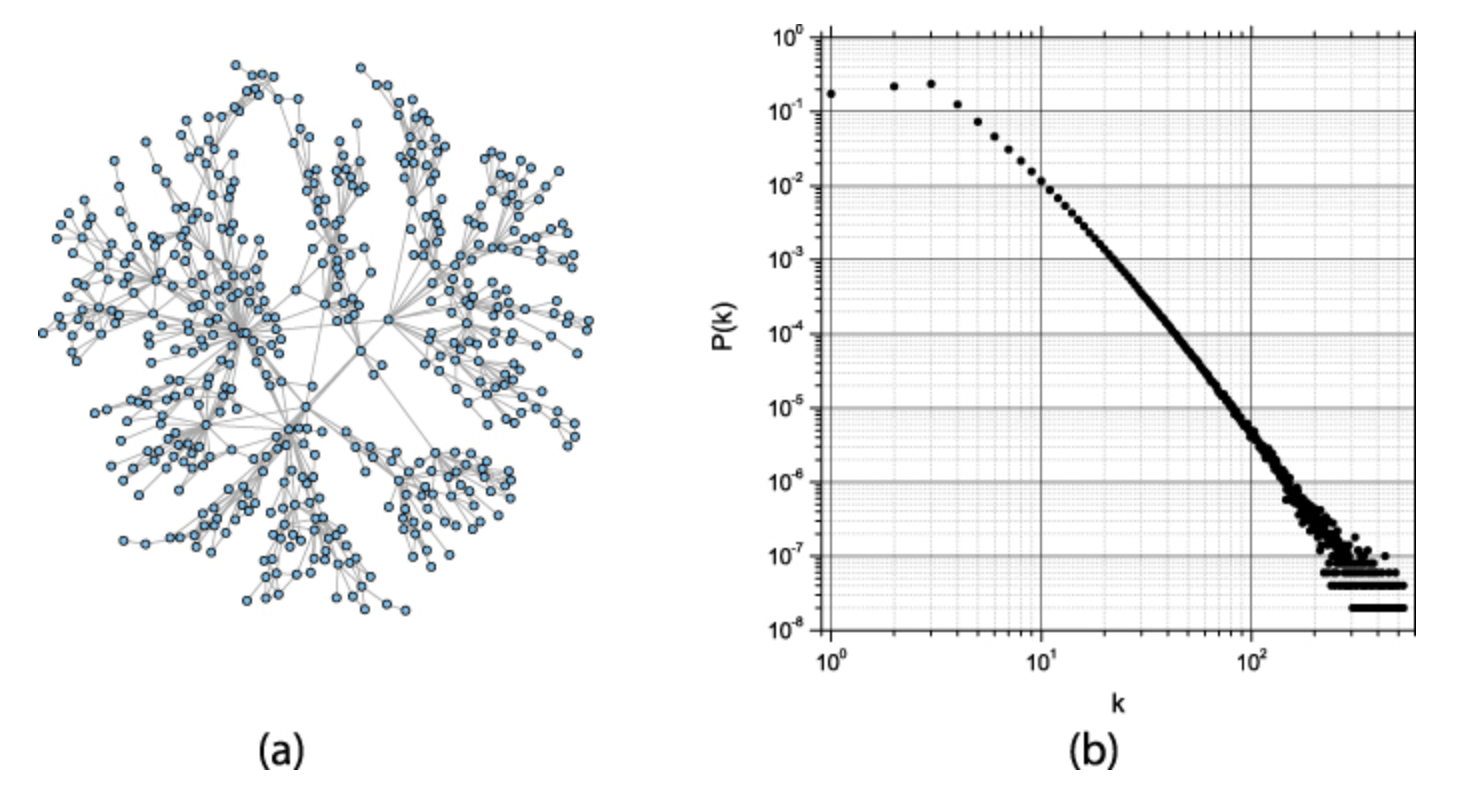
\includegraphics[width=\textwidth]{pl_example}
		  	\caption{\fullcite{Lubloy2008}} \label{fig:}
		  \end{figure}
		\end{frame}

	%%%%%%%%%%%%%%%%%%%%%%%%%%%%%%%%%%%%%%%%%%%%%%%%%%%%%%%%%%%%%%%%%%%%%%%%%%%%%%%%%%%%%%%%%%%
	%%%%%%%%%%%%%%%%%%%%%%%%%%%%%%%%%%%%%%%%%%%%%%%%%%%%%%%%%%%%%%%%%%%%%%%%%%%%%%%%%%%%%%%%%%%
		
		\begin{frame}\frametitle{Emergence of Scaling in Random Networks}
			\begin{figure}
				\centering
				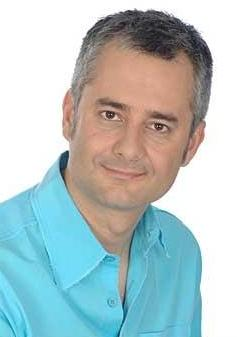
\includegraphics[width=.3\textwidth]{barabasicropped}
				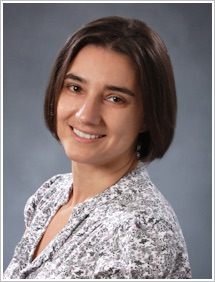
\includegraphics[width=.3\textwidth]{ralbert-photo}
			\end{figure}

			Albert-Laszlo Barabasi + Reka Albert (1999-2002); R.A.'s PhD thesis work.
			
			Central claim: \textbf{many real-world networks are scale-free.}
		\end{frame}

	%%%%%%%%%%%%%%%%%%%%%%%%%%%%%%%%%%%%%%%%%%%%%%%%%%%%%%%%%%%%%%%%%%%%%%%%%%%%%%%%%%%%%%%%%%%
	%%%%%%%%%%%%%%%%%%%%%%%%%%%%%%%%%%%%%%%%%%%%%%%%%%%%%%%%%%%%%%%%%%%%%%%%%%%%%%%%%%%%%%%%%%%
		
		\begin{frame}\frametitle{Emergence of Scaling in Random Networks\footfullcite{Barabasi1999}}

		\begin{figure}
			\centering
			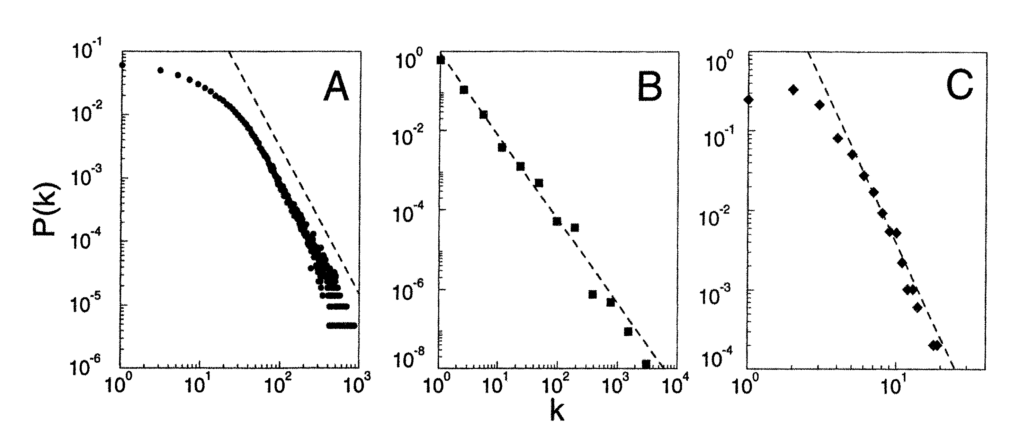
\includegraphics[width=\textwidth]{BA_data}
			\caption{(A) Actor collaboration graph $\gamma \approx 2.3$, (B) World Wide Web $\gamma \approx 2.1$, (C) Power grid network, $\gamma \approx 4$.}
		\end{figure}

		\end{frame}

	%%%%%%%%%%%%%%%%%%%%%%%%%%%%%%%%%%%%%%%%%%%%%%%%%%%%%%%%%%%%%%%%%%%%%%%%%%%%%%%%%%%%%%%%%%%
	%%%%%%%%%%%%%%%%%%%%%%%%%%%%%%%%%%%%%%%%%%%%%%%%%%%%%%%%%%%%%%%%%%%%%%%%%%%%%%%%%%%%%%%%%%%
		
		\begin{frame}\frametitle{Emergence of Scaling in Random Networks}
		  	
		  	\begin{block}{Empirical Claim}
		  		Many real networks have power law degree distributions with  $2 \leq \gamma \leq 3$.\footfullcite{Albert2002}
		  	\end{block}
		  	\begin{enumerate}
		  		\item Actor collaboration: $\gamma \approx 2.3$.
		  		\item World Wide Web: $\gamma \approx 2.1$.
		  		\item Protein interaction: $\gamma \approx 2.2-2.4$.
		  		\item Synonyms of words: $\gamma \approx 2.8$.
		  		\item \emph{Power grid: } $\gamma \approx 4$.
		  	\end{enumerate}
		\end{frame}
	%%%%%%%%%%%%%%%%%%%%%%%%%%%%%%%%%%%%%%%%%%%%%%%%%%%%%%%%%%%%%%%%%%%%%%%%%%%%%%%%%%%%%%%%%%%
	% %%%%%%%%%%%%%%%%%%%%%%%%%%%%%%%%%%%%%%%%%%%%%%%%%%%%%%%%%%%%%%%%%%%%%%%%%%%%%%%%%%%%%%%%%%%
		
	% 	\begin{frame}\frametitle{The Central Claim}
	% 	  	A common property of many large networks is that the vertex connectivities follow a scale-free power-law distribution. [The preferential attachment model] reproduces the observed stationary scale-free distributions, which indicates that the \emph{development of large networks is governed by robust self-organizing phenomena that go beyond the particulars of the individual systems.}\footfullcite{Eme1999}
	% 	\end{frame}
	
	% %%%%%%%%%%%%%%%%%%%%%%%%%%%%%%%%%%%%%%%%%%%%%%%%%%%%%%%%%%%%%%%%%%%%%%%%%%%%%%%%%%%%%%%%%%%
	%%%%%%%%%%%%%%%%%%%%%%%%%%%%%%%%%%%%%%%%%%%%%%%%%%%%%%%%%%%%%%%%%%%%%%%%%%%%%%%%%%%%%%%%%%%
		
		\begin{frame}\frametitle{Preferential Attachment Model (Barabasi-Albert)}
		  	\begin{enumerate}
		  		\item Initialize with a fixed graph $\mathcal{G}_0$. 
		  		\item At each time-step, add a node $v_t$ to $\mathcal{G}_{t-1}$. 
		  		\item Generate $m$ links between $v_t$ and $\mathcal{G}_{t-1}$, \emph{proportional to the degree of $\mathcal{G}$}. 
		  	\end{enumerate}
		  	\begin{align*}
		  		\prob(E = (v_t, v)) = \frac{d_v}{\sum_{u \in \mathcal{G}_{t-1}}d_u} 
		  	\end{align*}

		  	``The rich get richer.''
		\end{frame}
	
	%%%%%%%%%%%%%%%%%%%%%%%%%%%%%%%%%%%%%%%%%%%%%%%%%%%%%%%%%%%%%%%%%%%%%%%%%%%%%%%%%%%%%%%%%%%
	%%%%%%%%%%%%%%%%%%%%%%%%%%%%%%%%%%%%%%%%%%%%%%%%%%%%%%%%%%%%%%%%%%%%%%%%%%%%%%%%%%%%%%%%%%%
		
		\begin{frame}\frametitle{Properties of PA}
			For large $t$, 
			\begin{enumerate}
				\pause \item $\mathcal{G}_t$ has $t + \abs{\mathcal{G}_0}$ nodes. 
				\pause \item $\mathcal{G}_t$ mean degree $m$. 
				\pause \item The degree distribution $p_k$ is asymptotically power-law with exponent $\gamma = 3$ (can be generalized):
				\pause \begin{align}
				 	\prob(K_t = k) \propto k^{-3} \tag{asymptotic}.
				 \end{align} 
			\end{enumerate}
			\pause Proofs: master equations\footfullcite{Newman2010}, method of moments.\footfullcite{Dorogovtsev2000}
		\end{frame}
	
	%%%%%%%%%%%%%%%%%%%%%%%%%%%%%%%%%%%%%%%%%%%%%%%%%%%%%%%%%%%%%%%%%%%%%%%%%%%%%%%%%%%%%%%%%%%
	%%%%%%%%%%%%%%%%%%%%%%%%%%%%%%%%%%%%%%%%%%%%%%%%%%%%%%%%%%%%%%%%%%%%%%%%%%%%%%%%%%%%%%%%%%%
		
		\begin{frame}\frametitle{What's interesting about these networks?}
			\begin{block}{Empirical Claim}
		  		Many real networks have power law degree distributions with  $2 \leq \gamma \leq 3$.
		  	\end{block}
		  	Recall: 
			\begin{align}
				\E[K] &< \infty \iff \gamma > 2 \\ 
				\text{var} (K) &< \infty \iff \gamma > 3
			\end{align}
		  	What does this mean for phenomena governed by power laws? 
		\end{frame}
	
	%%%%%%%%%%%%%%%%%%%%%%%%%%%%%%%%%%%%%%%%%%%%%%%%%%%%%%%%%%%%%%%%%%%%%%%%%%%%%%%%%%%%%%%%%%%
	%%%%%%%%%%%%%%%%%%%%%%%%%%%%%%%%%%%%%%%%%%%%%%%%%%%%%%%%%%%%%%%%%%%%%%%%%%%%%%%%%%%%%%%%%%%
		
		\begin{frame}\frametitle{What's interesting about these networks?}
		  	\begin{itemize}
		  		\item Scale-free networks are ``\textbf{ultrasmall}''\footfullcite{Cohen2003a}: $D \sim \log \log n$. 
		  		\item Scale-free networks have no \textbf{epidemic threshold}: Any rumor, no matter how silly, has nonzero probability to spread through a large proportion of a scalefree network.\footfullcite{Pastor-Satorras2001a}
		  		\item Scale-free networks are \textbf{robust} to random failure.\footfullcite{Albert2004}
		  	\end{itemize}
		\end{frame}
	
	%%%%%%%%%%%%%%%%%%%%%%%%%%%%%%%%%%%%%%%%%%%%%%%%%%%%%%%%%%%%%%%%%%%%%%%%%%%%%%%%%%%%%%%%%%%
	%%%%%%%%%%%%%%%%%%%%%%%%%%%%%%%%%%%%%%%%%%%%%%%%%%%%%%%%%%%%%%%%%%%%%%%%%%%%%%%%%%%%%%%%%%%
		
		\begin{frame}\frametitle{More Models of Scale-Free Networks}
			\begin{itemize}
				\item Preferential attachment model. 
				\item Configuration model (exact degree sequence).
				\item Chung-Lu model (expected degrees).\footfullcite{Chung2002} 
				\item Vertex-copying model.\footfullcite{Kleinberg1999}
			\end{itemize}
		\end{frame}
	
	%%%%%%%%%%%%%%%%%%%%%%%%%%%%%%%%%%%%%%%%%%%%%%%%%%%%%%%%%%%%%%%%%%%%%%%%%%%%%%%%%%%%%%%%%%%
	%%%%%%%%%%%%%%%%%%%%%%%%%%%%%%%%%%%%%%%%%%%%%%%%%%%%%%%%%%%%%%%%%%%%%%%%%%%%%%%%%%%%%%%%%%%
		
		\begin{frame}\frametitle{A Theory of Everything for Networks?}
			\begin{columns}
				\begin{column}{.35\textwidth}
				\begin{figure}
					\centering
						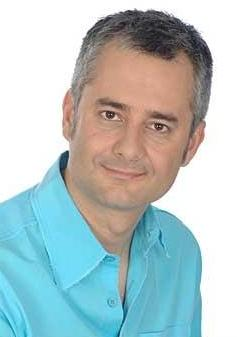
\includegraphics[width=.9\textwidth]{barabasicropped}
					\caption{} \label{fig:}
				\end{figure}
					
				\end{column}
				\begin{column}{.65\textwidth}
				  	``Yet, probably the most surprising discovery of modern network theory is the \emph{universality of the network topology}: Many real networks, from the cell to the Internet, independent of their age, function, and scope, converge to similar architectures. \emph{It is this universality that allowed researchers from different disciplines to embrace network theory as a common paradigm}.''
			  	\end{column}
		  	\end{columns}
		  	\color{white}{\footfullcite{Barabasi2009}}
		\end{frame}
	%%%%%%%%%%%%%%%%%%%%%%%%%%%%%%%%%%%%%%%%%%%%%%%%%%%%%%%%%%%%%%%%%%%%%%%%%%%%%%%%%%%%%%%%%%%
	%%%%%%%%%%%%%%%%%%%%%%%%%%%%%%%%%%%%%%%%%%%%%%%%%%%%%%%%%%%%%%%%%%%%%%%%%%%%%%%%%%%%%%%%%%%
		
		\begin{frame}\frametitle{Emergence of Citations of ``Emergence of Scaling''}
			Imagine writing your PhD thesis...
			\begin{itemize}
				\pause \item ...and having it published in \emph{Nature}, \emph{Science}, and \emph{Physical Review Letters}...
				\pause \item ...and being cited \textbf{70,000} times....  
				\pause \item ...10 times per day, for almost 20 years. 
				\pause \item In expectation, there will be a paper published that cites their work \textbf{\emph{during this talk.}}
			\end{itemize}
			\pause R. Albert is now a Distinguished Prof. at Penn State. Barabasi is the \textbf{5th most cited physicist} on Google Scholar. 
		\end{frame}
	
	%%%%%%%%%%%%%%%%%%%%%%%%%%%%%%%%%%%%%%%%%%%%%%%%%%%%%%%%%%%%%%%%%%%%%%%%%%%%%%%%%%%%%%%%%%%
		
		\begin{frame}\frametitle{A Tidy Picture}
		  	\begin{itemize}
		  		\item \textbf{Theory}: We have many models of how scale-free networks emerge. 
		  		\item \textbf{Theory}: We have many interesting theoretical properties of scale-free networks. 
		  		\item \textbf{Data}: We have many papers observing power laws in real-world data...right? 
		  	\end{itemize}
		\end{frame}
	
	%%%%%%%%%%%%%%%%%%%%%%%%%%%%%%%%%%%%%%%%%%%%%%%%%%%%%%%%%%%%%%%%%%%%%%%%%%%%%%%%%%%%%%%%%%%
	%%%%%%%%%%%%%%%%%%%%%%%%%%%%%%%%%%%%%%%%%%%%%%%%%%%%%%%%%%%%%%%%%%%%%%%%%%%%%%%%%%%%%%%%%%%
		
		\begin{frame}\frametitle{Well...}
			\begin{columns}
				\begin{column}{.35 \textwidth}
					\begin{figure}
						\centering
						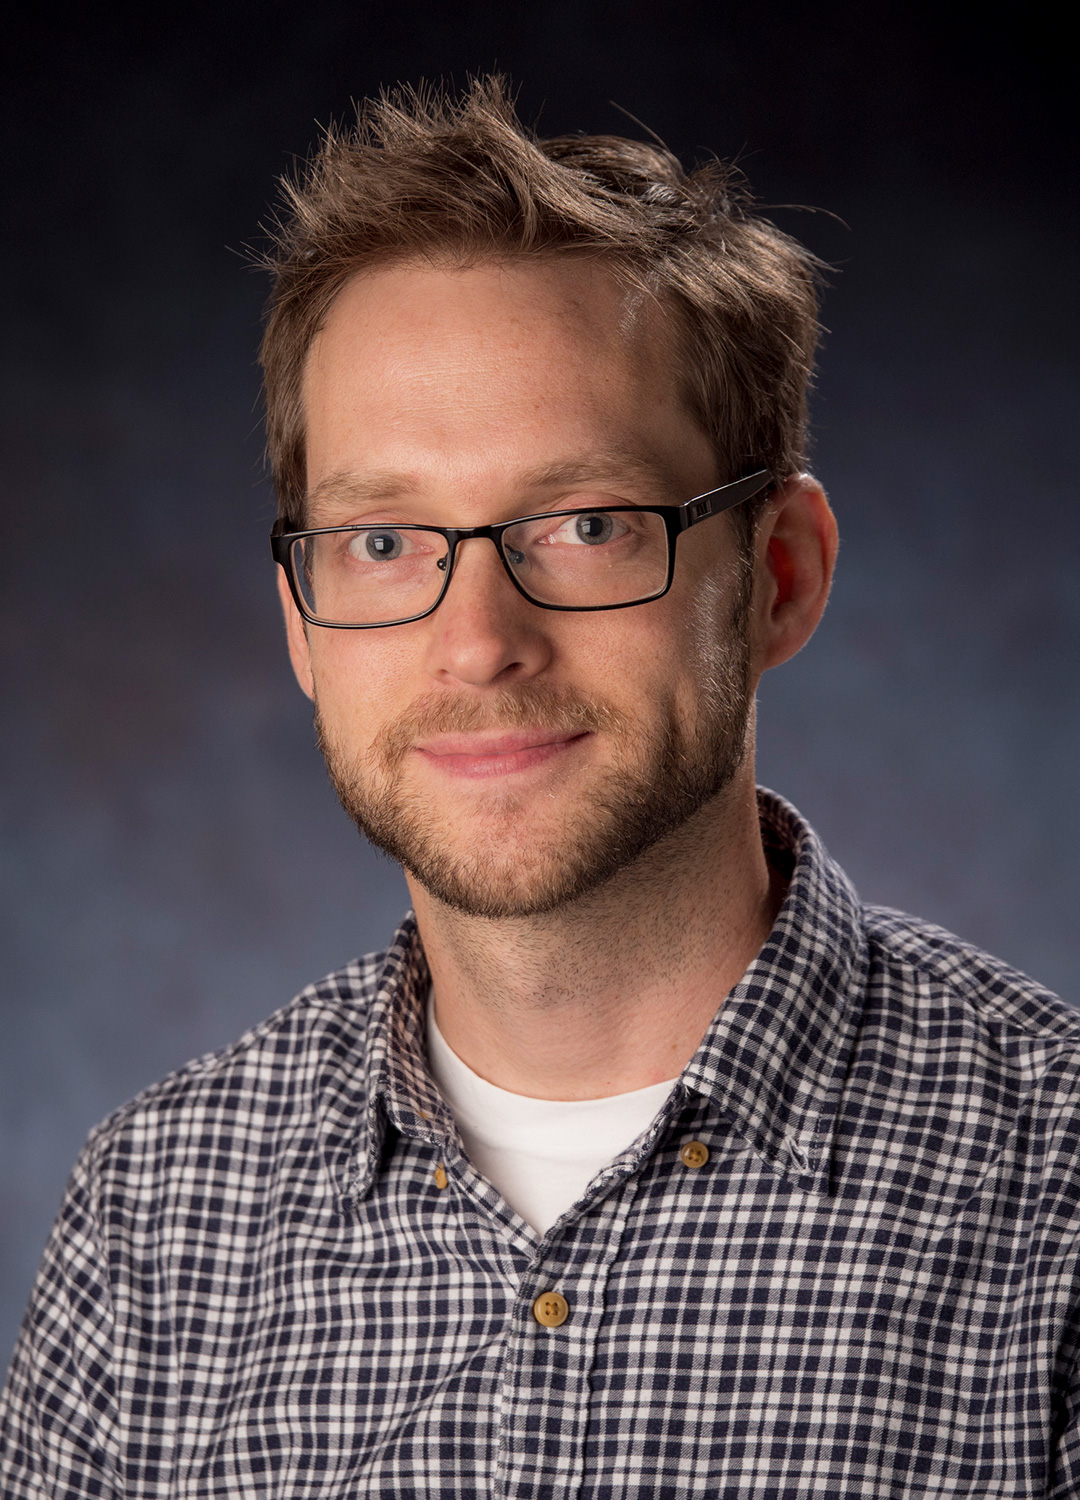
\includegraphics[width=.9\textwidth]{AaronClauset_1500}
						\caption{Aaron Clauset, UC Boulder} \label{fig:}
					\end{figure}
				\end{column}
				\begin{column}{.65\textwidth}
					``There must be a thousand papers in which people plot the degree distribution, put a line through it and say it’s scale-free without really doing the careful statistical work.''
				\end{column}
			\end{columns}
			\color{white}{\footnote{Quanta: "Scant Evidence of Power Laws Found in Real-World Networks."}}
		\end{frame}
	%%%%%%%%%%%%%%%%%%%%%%%%%%%%%%%%%%%%%%%%%%%%%%%%%%%%%%%%%%%%%%%%%%%%%%%%%%%%%%%%%%%%%%%%%%%
\section{Measuring Power Laws}
	%%%%%%%%%%%%%%%%%%%%%%%%%%%%%%%%%%%%%%%%%%%%%%%%%%%%%%%%%%%%%%%%%%%%%%%%%%%%%%%%%%%%%%%%%%%
		
		\begin{frame}\frametitle{The Problem with Log-Log Plots...}
		Empirical CDF of 100 samples from a degree distribution. How many are power laws?
		\begin{figure}
			\centering
				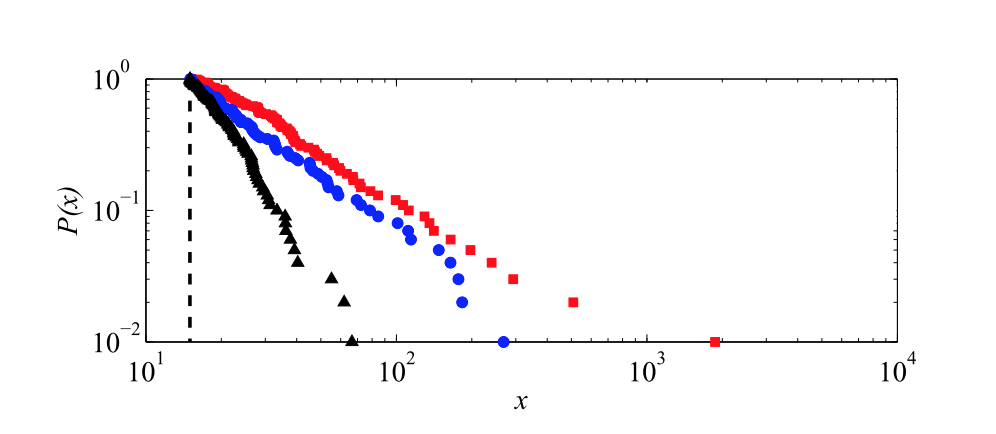
\includegraphics[width=\textwidth]{4_1_censored}
			\caption{\tiny{\fullcite{Clauset2009}}} 
		\end{figure}
		  	
		\end{frame}

	%%%%%%%%%%%%%%%%%%%%%%%%%%%%%%%%%%%%%%%%%%%%%%%%%%%%%%%%%%%%%%%%%%%%%%%%%%%%%%%%%%%%%%%%%%%
	%%%%%%%%%%%%%%%%%%%%%%%%%%%%%%%%%%%%%%%%%%%%%%%%%%%%%%%%%%%%%%%%%%%%%%%%%%%%%%%%%%%%%%%%%%%
		
		\begin{frame}\frametitle{The Problem with Log-Log Plots...}
		Empirical CDF of 100 samples from a degree distribution. How many are power laws?
		  	\begin{figure}
			\centering
				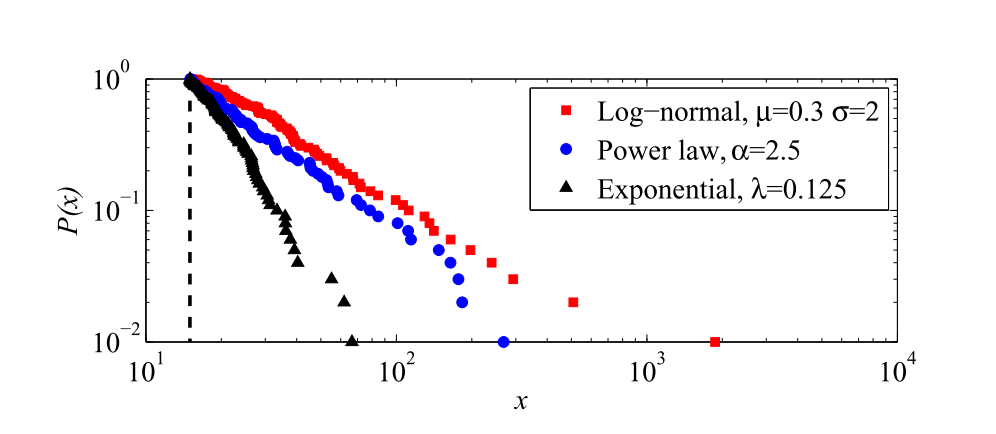
\includegraphics[width=\textwidth]{4_1}
			\caption{\tiny{\fullcite{Clauset2009}}} 
		\end{figure}
		\end{frame}

	%%%%%%%%%%%%%%%%%%%%%%%%%%%%%%%%%%%%%%%%%%%%%%%%%%%%%%%%%%%%%%%%%%%%%%%%%%%%%%%%%%%%%%%%%%%
	%%%%%%%%%%%%%%%%%%%%%%%%%%%%%%%%%%%%%%%%%%%%%%%%%%%%%%%%%%%%%%%%%%%%%%%%%%%%%%%%%%%%%%%%%%%
		
		\begin{frame}\frametitle{We need statistics...}
		  	\begin{block}{Inference}
		  		What are the power law parameters that best fit the data? 
		  	\end{block}
		  	\begin{block}{Model Evaluation}
		  		Is the power law a plausible model of the data at all?
		  	\end{block}
		\end{frame}
	
	%%%%%%%%%%%%%%%%%%%%%%%%%%%%%%%%%%%%%%%%%%%%%%%%%%%%%%%%%%%%%%%%%%%%%%%%%%%%%%%%%%%%%%%%%%%
	%%%%%%%%%%%%%%%%%%%%%%%%%%%%%%%%%%%%%%%%%%%%%%%%%%%%%%%%%%%%%%%%%%%%%%%%%%%%%%%%%%%%%%%%%%%
		
		\begin{frame}\frametitle{``Scale Free Networks are Rare''}
		  	\begin{figure}
				\centering
				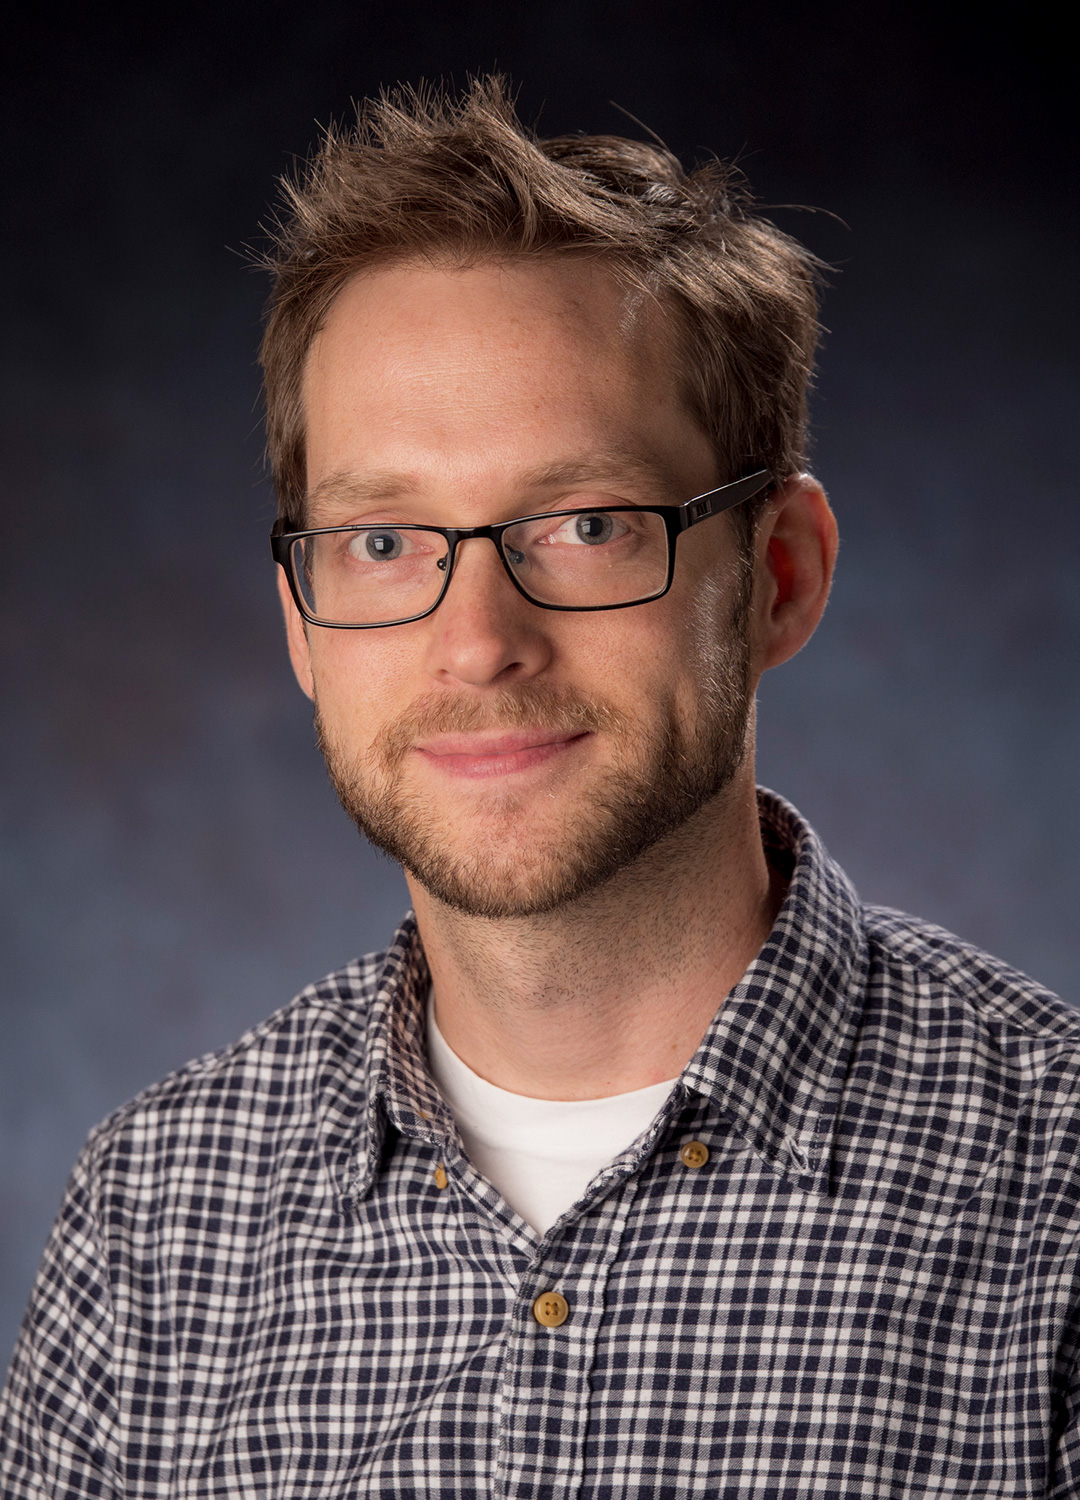
\includegraphics[width=.3\textwidth]{AaronClauset_1500}
				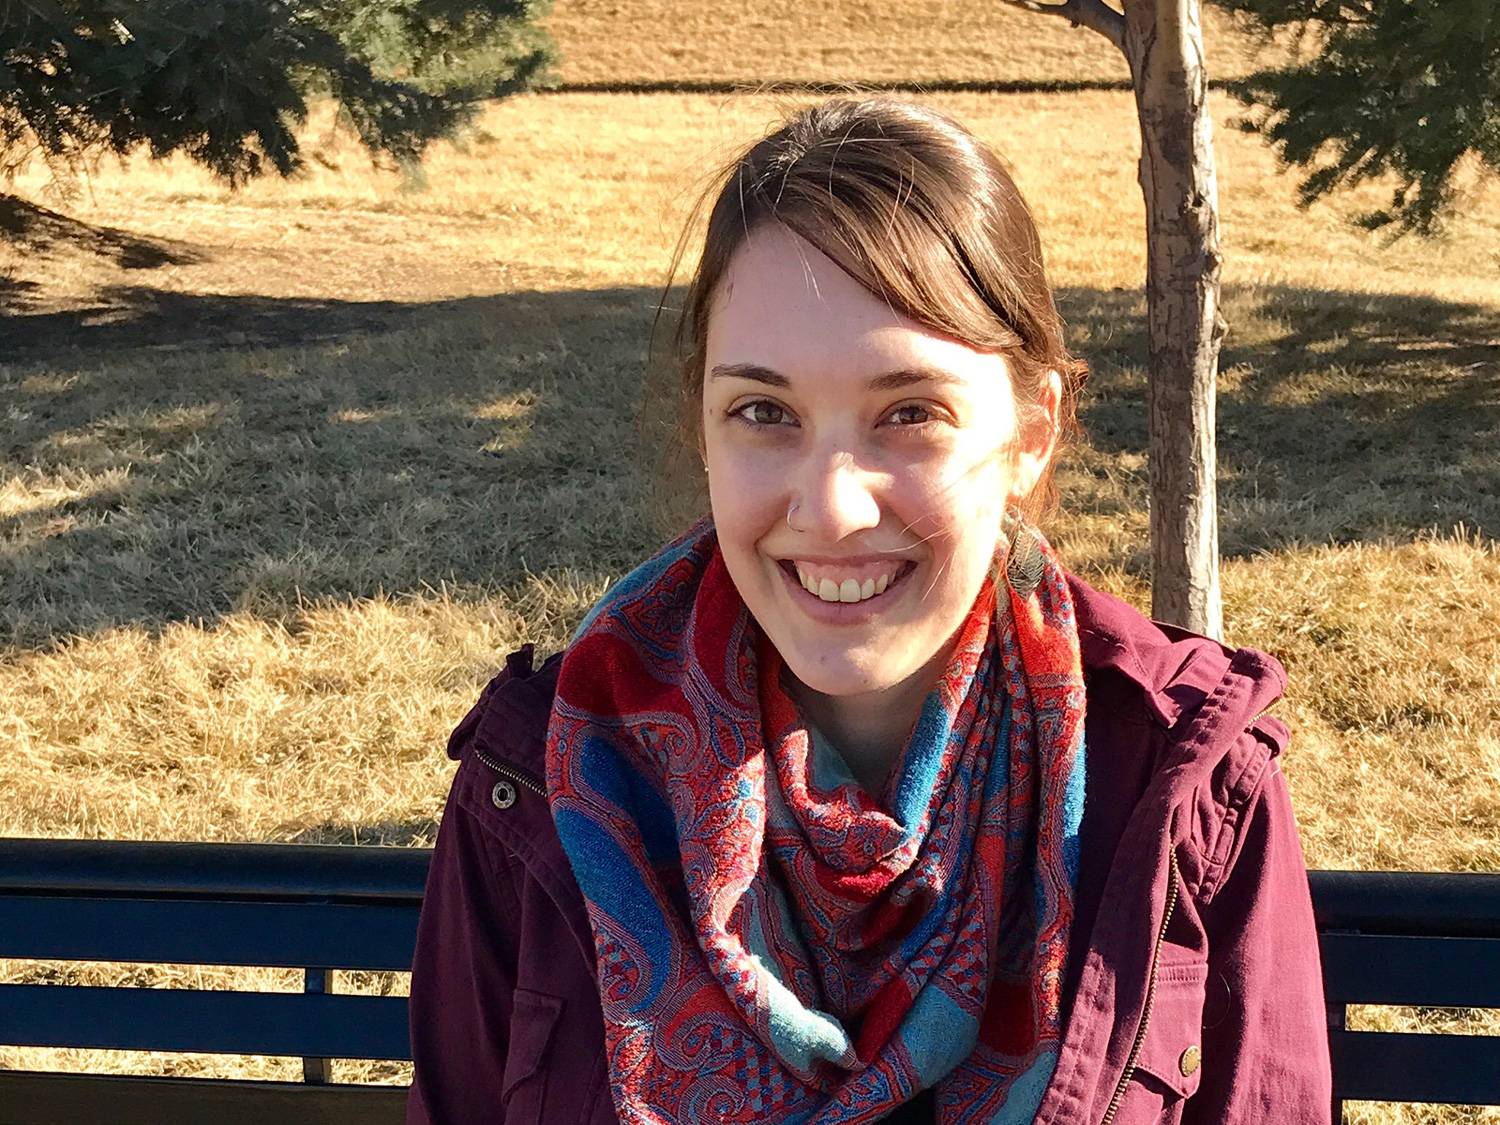
\includegraphics[width=.55\textwidth]{AnnaBroido}
			\end{figure}
			\color{white}{\footfullcite{Broido2017}}
		\end{frame}
	
	%%%%%%%%%%%%%%%%%%%%%%%%%%%%%%%%%%%%%%%%%%%%%%%%%%%%%%%%%%%%%%%%%%%%%%%%%%%%%%%%%%%%%%%%%%%
	%%%%%%%%%%%%%%%%%%%%%%%%%%%%%%%%%%%%%%%%%%%%%%%%%%%%%%%%%%%%%%%%%%%%%%%%%%%%%%%%%%%%%%%%%%%
		
		\begin{frame}\frametitle{Methodology}
		  	\begin{enumerate}
		  		\item Collect large set of network data sets.\footnote{\url{https://icon.colorado.edu/}}
		  		\item For each data set, perform inference and model evaluation as described above. 
		  		\item \textbf{Compare} power law to a set of alternative models (exponential, log-normal, etc) using an \emph{likelihood ratio test}.  
		  	\end{enumerate}
		\end{frame}
	
	%%%%%%%%%%%%%%%%%%%%%%%%%%%%%%%%%%%%%%%%%%%%%%%%%%%%%%%%%%%%%%%%%%%%%%%%%%%%%%%%%%%%%%%%%%%
	%%%%%%%%%%%%%%%%%%%%%%%%%%%%%%%%%%%%%%%%%%%%%%%%%%%%%%%%%%%%%%%%%%%%%%%%%%%%%%%%%%%%%%%%%%%
		
		\begin{frame}\frametitle{Some Startling Findings}
			\begin{enumerate}
				\item For $573 / 882 = 65\%$ of data sets, power law is either implausible or worse than a simple alternative model. 
				\item For only 11\% of data sets is a power law plausible, clearly favored over simple alternatives, and displays $2 \leq \gamma \leq 3$.
			\end{enumerate}
		\end{frame}
	
	%%%%%%%%%%%%%%%%%%%%%%%%%%%%%%%%%%%%%%%%%%%%%%%%%%%%%%%%%%%%%%%%%%%%%%%%%%%%%%%%%%%%%%%%%%%
	%%%%%%%%%%%%%%%%%%%%%%%%%%%%%%%%%%%%%%%%%%%%%%%%%%%%%%%%%%%%%%%%%%%%%%%%%%%%%%%%%%%%%%%%%%%
		
		\begin{frame}\frametitle{But...}
			Even ground-truth preferential attachment networks fail many of Broido + Clauset's tests...

			\emph{When we consider the plausibility of the power-law fit, we see fewer networks. 62\% of the preferential attachment graphs fall into the Weakest and Weak categories, 60\% in the Strong category, and 0 in the Strongest category.}
		\end{frame}
	
	%%%%%%%%%%%%%%%%%%%%%%%%%%%%%%%%%%%%%%%%%%%%%%%%%%%%%%%%%%%%%%%%%%%%%%%%%%%%%%%%%%%%%%%%%%%
	%%%%%%%%%%%%%%%%%%%%%%%%%%%%%%%%%%%%%%%%%%%%%%%%%%%%%%%%%%%%%%%%%%%%%%%%%%%%%%%%%%%%%%%%%%%
		
		\begin{frame}\frametitle{Ongoing Debate...}
		  	
		  	\begin{columns}
				\begin{column}{.35\textwidth}
				\begin{figure}
					\centering
						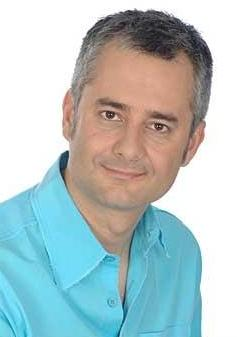
\includegraphics[width=.9\textwidth]{barabasicropped}
					\caption{} \label{fig:}
				\end{figure}
					
				\end{column}
				\begin{column}{.65\textwidth}
				  	``...You will find that the study is oblivious to 18 years of knowledge accumulated in network science. You will also find a fictional criterion of scale-free networks. Most important, you will find that their central criterion of scale-freeness fails the most elementary tests. And those are only the big problems...''
			  	\end{column}
		  	\end{columns}

		\end{frame}
	
	%%%%%%%%%%%%%%%%%%%%%%%%%%%%%%%%%%%%%%%%%%%%%%%%%%%%%%%%%%%%%%%%%%%%%%%%%%%%%%%%%%%%%%%%%%%
	%%%%%%%%%%%%%%%%%%%%%%%%%%%%%%%%%%%%%%%%%%%%%%%%%%%%%%%%%%%%%%%%%%%%%%%%%%%%%%%%%%%%%%%%%%%
		
		\begin{frame}\frametitle{The Next Chapter...?}
			\centering
			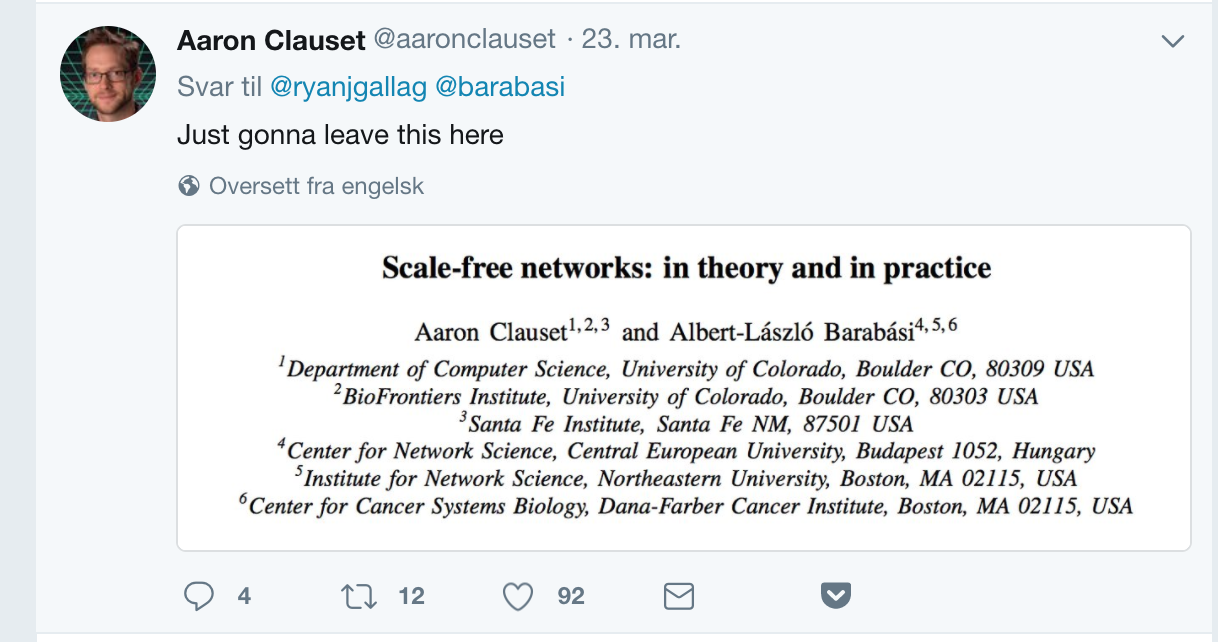
\includegraphics[width=\textwidth]{twitter_reconciliation}
		\end{frame}
	
	%%%%%%%%%%%%%%%%%%%%%%%%%%%%%%%%%%%%%%%%%%%%%%%%%%%%%%%%%%%%%%%%%%%%%%%%%%%%%%%%%%%%%%%%%%%
	%%%%%%%%%%%%%%%%%%%%%%%%%%%%%%%%%%%%%%%%%%%%%%%%%%%%%%%%%%%%%%%%%%%%%%%%%%%%%%%%%%%%%%%%%%%
		
		\begin{frame}[standout]
		  	Thanks!
		\end{frame}
	
	%%%%%%%%%%%%%%%%%%%%%%%%%%%%%%%%%%%%%%%%%%%%%%%%%%%%%%%%%%%%%%%%%%%%%%%%%%%%%%%%%%%%%%%%%%%
\end{document}
